% GENERATED FILE - do not hand-edit.
% Source of truth: data/calculus-reviewed/c-4.json in the zenith-website repo.
% Regenerate with: python3 scripts/build_calculus_tex.py
\documentclass[11pt]{article}
\usepackage[utf8]{inputenc}
\usepackage[T1]{fontenc}
\usepackage{amsmath,amssymb}
\usepackage{graphicx}
\usepackage[margin=1in]{geometry}
\graphicspath{{../..//}}
\setlength{\parindent}{0pt}
\setlength{\parskip}{0.6em}
\begin{document}
\section*{Chapter 4: Application of Differential Calculus --- Practice Exercises C4}

\bigskip\noindent\textbf{A1.}\ The slope of the curve $y^3 - xy^2 = 4$ at the point where $y=2$ is
\begin{list}{}{\setlength{\leftmargin}{3em}\setlength{\labelwidth}{2.5em}\setlength{\itemsep}{0pt}\setlength{\topsep}{2pt}}
\item[(A)] $-2$
\item[(B)] $-\frac12$
\item[(C)] $\frac12$
\item[(D)] $2$
\end{list}

\bigskip\noindent\textbf{A2.}\ The slope of the curve $y^2 - xy - 3x = 1$ at the point $(0,-1)$ is
\begin{list}{}{\setlength{\leftmargin}{3em}\setlength{\labelwidth}{2.5em}\setlength{\itemsep}{0pt}\setlength{\topsep}{2pt}}
\item[(A)] $-1$
\item[(B)] $-2$
\item[(C)] $1$
\item[(D)] $2$
\end{list}

\bigskip\noindent\textbf{A3.}\ An equation of the tangent to $y=x\sin x$ at $(\pi/2,\pi/2)$ is
\begin{list}{}{\setlength{\leftmargin}{3em}\setlength{\labelwidth}{2.5em}\setlength{\itemsep}{0pt}\setlength{\topsep}{2pt}}
\item[(A)] $y=x-\pi$
\item[(B)] $y=\frac\pi2$
\item[(C)] $y=\pi-x$
\item[(D)] $y=x$
\end{list}

\bigskip\noindent\textbf{A4.}\ The tangent to the curve of $y = xe^{-x}$ is horizontal when $x$ is equal to
\begin{list}{}{\setlength{\leftmargin}{3em}\setlength{\labelwidth}{2.5em}\setlength{\itemsep}{0pt}\setlength{\topsep}{2pt}}
\item[(A)] $0$
\item[(B)] $1$
\item[(C)] $-1$
\item[(D)] $\frac1e$
\end{list}

\bigskip\noindent\textbf{A5.}\ The minimum value of the slope of the curve $y = x^5 + x^3 - 2x$ is
\begin{list}{}{\setlength{\leftmargin}{3em}\setlength{\labelwidth}{2.5em}\setlength{\itemsep}{0pt}\setlength{\topsep}{2pt}}
\item[(A)] $2$
\item[(B)] $6$
\item[(C)] $-2$
\item[(D)] $-6$
\end{list}

\bigskip\noindent\textbf{A6.}\ An equation of the tangent to the hyperbola $x^2-y^2=12$ at $(4,2)$ is
\begin{list}{}{\setlength{\leftmargin}{3em}\setlength{\labelwidth}{2.5em}\setlength{\itemsep}{0pt}\setlength{\topsep}{2pt}}
\item[(A)] $x-2y+6=0$
\item[(B)] $y=2x$
\item[(C)] $y=2x-6$
\item[(D)] $y=\frac x2$
\end{list}

\bigskip\noindent\textbf{A7.}\ A tangent to the curve $y^2-xy+9=0$ is vertical when
\begin{list}{}{\setlength{\leftmargin}{3em}\setlength{\labelwidth}{2.5em}\setlength{\itemsep}{0pt}\setlength{\topsep}{2pt}}
\item[(A)] $y=0$
\item[(B)] $y=\pm\sqrt3$
\item[(C)] $y=\frac12$
\item[(D)] $y=\pm3$
\end{list}

\bigskip\noindent\textbf{A8.}\ The volume of a sphere is given by $V = \frac{4}{3}\pi r^3$. Use a tangent line to approximate the increase in volume, in cubic inches, when the radius of a sphere is increased from 3 to 3.1 inches.
\begin{list}{}{\setlength{\leftmargin}{3em}\setlength{\labelwidth}{2.5em}\setlength{\itemsep}{0pt}\setlength{\topsep}{2pt}}
\item[(A)] $\frac{0.04\pi}3$
\item[(B)] $0.04\pi$
\item[(C)] $1.2\pi$
\item[(D)] $3.6\pi$
\end{list}

\bigskip\noindent\textbf{A9.}\ When $x=3$, the equation $2x^2-y^3=10$ has the solution $y=2$. Using a tangent line to the graph of the curve, approximate $y$ when $x=3.04$.
\begin{list}{}{\setlength{\leftmargin}{3em}\setlength{\labelwidth}{2.5em}\setlength{\itemsep}{0pt}\setlength{\topsep}{2pt}}
\item[(A)] $1.6$
\item[(B)] $1.96$
\item[(C)] $2.04$
\item[(D)] $2.4$
\end{list}

\bigskip\noindent\textbf{A10.}\ If the side $e$ of a square is increased by 1\%, then the area is increased approximately
\begin{list}{}{\setlength{\leftmargin}{3em}\setlength{\labelwidth}{2.5em}\setlength{\itemsep}{0pt}\setlength{\topsep}{2pt}}
\item[(A)] $0.02e$
\item[(B)] $0.02e^2$
\item[(C)] $0.01e^2$
\item[(D)] $0.01e$
\end{list}

\bigskip\noindent\textbf{A11.}\ The edge of a cube has length 10 in., with a possible error of 1\%. The possible error, in cubic inches, in the volume of the cube is
\begin{list}{}{\setlength{\leftmargin}{3em}\setlength{\labelwidth}{2.5em}\setlength{\itemsep}{0pt}\setlength{\topsep}{2pt}}
\item[(A)] $1$
\item[(B)] $3$
\item[(C)] $10$
\item[(D)] $30$
\end{list}

\bigskip\noindent\textbf{A12.}\ The function $f(x) = x^4 - 4x^2$ has
\begin{list}{}{\setlength{\leftmargin}{3em}\setlength{\labelwidth}{2.5em}\setlength{\itemsep}{0pt}\setlength{\topsep}{2pt}}
\item[(A)] one local minimum and two local maxima
\item[(B)] one local minimum and no local maximum
\item[(C)] no local minimum and one local maximum
\item[(D)] two local minima and one local maximum
\end{list}

\bigskip\noindent\textbf{A13.}\ The number of inflection points on the graph of $f(x) = x^4 - 4x^2$ is
\begin{list}{}{\setlength{\leftmargin}{3em}\setlength{\labelwidth}{2.5em}\setlength{\itemsep}{0pt}\setlength{\topsep}{2pt}}
\item[(A)] $0$
\item[(B)] $1$
\item[(C)] $2$
\item[(D)] $3$
\end{list}

\bigskip\noindent\textbf{A14.}\ The maximum value of the function $y = -4\sqrt{2-x}$ is
\begin{list}{}{\setlength{\leftmargin}{3em}\setlength{\labelwidth}{2.5em}\setlength{\itemsep}{0pt}\setlength{\topsep}{2pt}}
\item[(A)] $0$
\item[(B)] $-4$
\item[(C)] $-2$
\item[(D)] $2$
\end{list}

\bigskip\noindent\textbf{A15.}\ The total number of local maximum and minimum points of the function whose derivative, for all $x$, is given by $f'(x) = x(x-3)^2(x+1)^4$ is
\begin{list}{}{\setlength{\leftmargin}{3em}\setlength{\labelwidth}{2.5em}\setlength{\itemsep}{0pt}\setlength{\topsep}{2pt}}
\item[(A)] $0$
\item[(B)] $1$
\item[(C)] $2$
\item[(D)] $3$
\end{list}

\bigskip\noindent\textbf{A16.}\ For which curve shown below are both $f'$ and $f''$ negative?
\begin{center}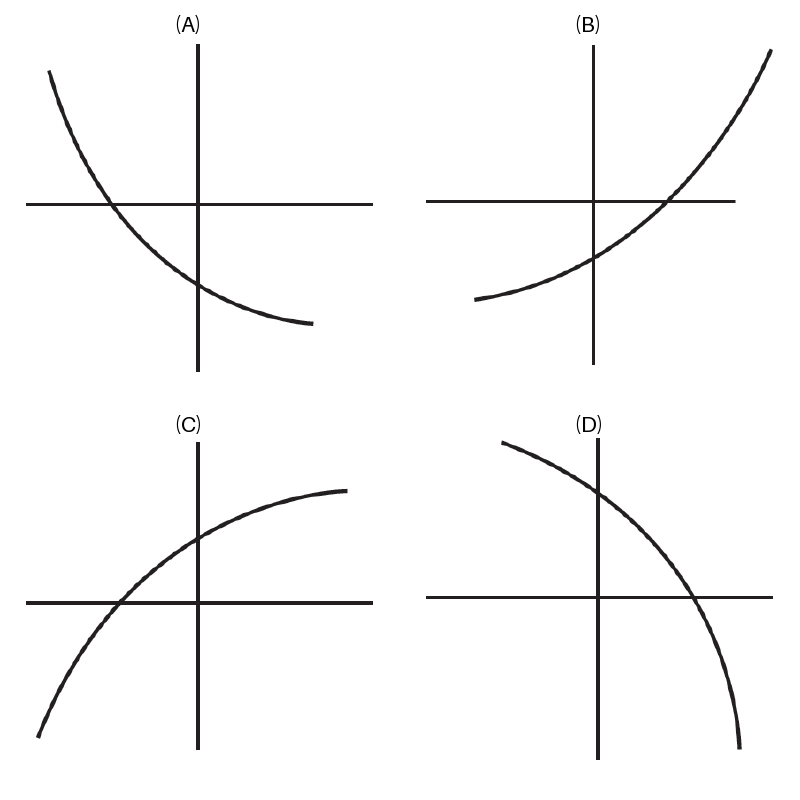
\includegraphics[width=0.6\linewidth]{data/calculus-figures/c4-curves.png}\end{center}
\begin{list}{}{\setlength{\leftmargin}{3em}\setlength{\labelwidth}{2.5em}\setlength{\itemsep}{0pt}\setlength{\topsep}{2pt}}
\item[(A)] Curve (A)
\item[(B)] Curve (B)
\item[(C)] Curve (C)
\item[(D)] Curve (D)
\end{list}

\bigskip\noindent\textbf{A17.}\ For which curve shown below is $f\prime\prime$ positive but $f\prime$ negative?
\begin{center}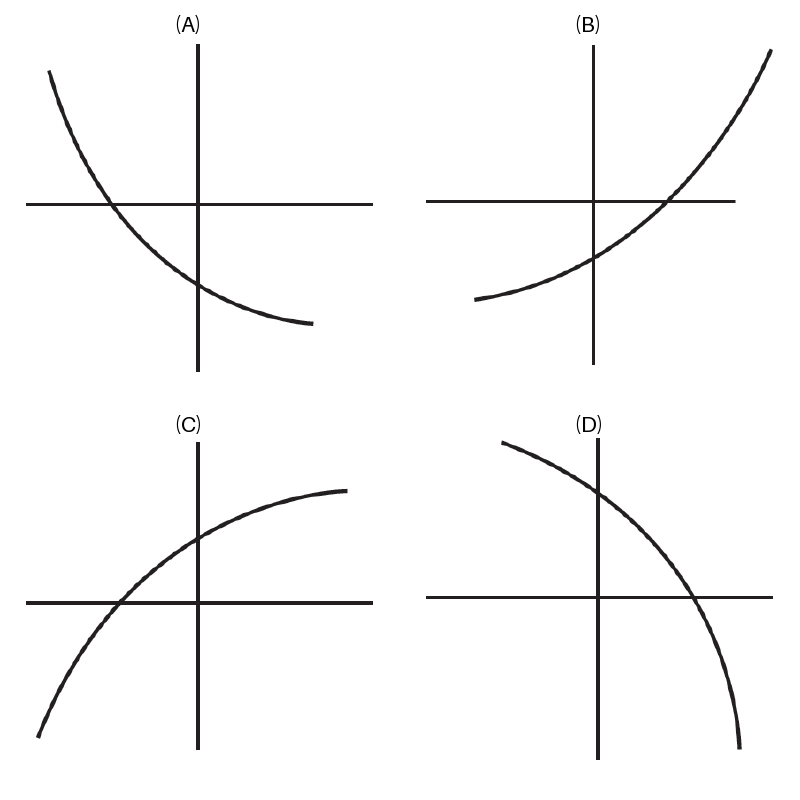
\includegraphics[width=0.6\linewidth]{data/calculus-figures/c4-curves.png}\end{center}
\begin{list}{}{\setlength{\leftmargin}{3em}\setlength{\labelwidth}{2.5em}\setlength{\itemsep}{0pt}\setlength{\topsep}{2pt}}
\item[(A)] Curve (A)
\item[(B)] Curve (B)
\item[(C)] Curve (C)
\item[(D)] Curve (D)
\end{list}

\bigskip\noindent\textbf{A18.}\ The position of a particle moving along a horizontal line is $s=t^3-6t^2+12t-8$. The object is moving to the right for
\begin{list}{}{\setlength{\leftmargin}{3em}\setlength{\labelwidth}{2.5em}\setlength{\itemsep}{0pt}\setlength{\topsep}{2pt}}
\item[(A)] $t < 2$
\item[(B)] all $t$ except $t=2$
\item[(C)] all $t$
\item[(D)] $t>2$
\end{list}

\bigskip\noindent\textbf{A19.}\ The position of a particle moving along a horizontal line is $s=t^3-6t^2+12t-8$. The minimum value of the speed is
\begin{list}{}{\setlength{\leftmargin}{3em}\setlength{\labelwidth}{2.5em}\setlength{\itemsep}{0pt}\setlength{\topsep}{2pt}}
\item[(A)] $0$
\item[(B)] $1$
\item[(C)] $2$
\item[(D)] $3$
\end{list}

\bigskip\noindent\textbf{A20.}\ The position of a particle moving along a horizontal line is $s=t^3-6t^2+12t-8$. The acceleration is positive
\begin{list}{}{\setlength{\leftmargin}{3em}\setlength{\labelwidth}{2.5em}\setlength{\itemsep}{0pt}\setlength{\topsep}{2pt}}
\item[(A)] when $t>2$
\item[(B)] for all $t$, $t \neq 2$
\item[(C)] when $t<2$
\item[(D)] for $1<t<2$
\end{list}

\bigskip\noindent\textbf{A21.}\ The position of a particle moving along a horizontal line is $s=t^3-6t^2+12t-8$. The speed of the particle is decreasing for
\begin{list}{}{\setlength{\leftmargin}{3em}\setlength{\labelwidth}{2.5em}\setlength{\itemsep}{0pt}\setlength{\topsep}{2pt}}
\item[(A)] $t<2$
\item[(B)] all $t$
\item[(C)] $t<1$ or $t>2$
\item[(D)] $t>2$
\end{list}

\bigskip\noindent\textbf{A22.}\ A particle moves along a horizontal line with position $s=t^4-6t^3+12t^2+3$ at time $t$. The particle is at rest when $t$ is equal to
\begin{list}{}{\setlength{\leftmargin}{3em}\setlength{\labelwidth}{2.5em}\setlength{\itemsep}{0pt}\setlength{\topsep}{2pt}}
\item[(A)] $1$ or $2$
\item[(B)] $0$
\item[(C)] $\frac94$
\item[(D)] $0$, $1$, or $2$
\end{list}

\bigskip\noindent\textbf{A23.}\ A particle moves along a horizontal line with position $s=t^4-6t^3+12t^2+3$ at time $t$. The velocity, $v$, is increasing when
\begin{list}{}{\setlength{\leftmargin}{3em}\setlength{\labelwidth}{2.5em}\setlength{\itemsep}{0pt}\setlength{\topsep}{2pt}}
\item[(A)] $t>1$
\item[(B)] $1<t<2$
\item[(C)] $t<2$
\item[(D)] $t<1$ or $t>2$
\end{list}

\bigskip\noindent\textbf{A24.}\ A particle moves along a horizontal line with position $s=t^4-6t^3+12t^2+3$ at time $t$. The speed of the particle is increasing for
\begin{list}{}{\setlength{\leftmargin}{3em}\setlength{\labelwidth}{2.5em}\setlength{\itemsep}{0pt}\setlength{\topsep}{2pt}}
\item[(A)] $0<t<1$ or $t>2$
\item[(B)] $1<t<2$
\item[(C)] $t<2$
\item[(D)] $t<0$ or $t>2$
\end{list}

\bigskip\noindent\textbf{A25.}\ The displacement from the origin of a particle moving on a line is given by $s = t^4-4t^3$. The maximum displacement during the time interval $-2 \leq t \leq 4$ is
\begin{list}{}{\setlength{\leftmargin}{3em}\setlength{\labelwidth}{2.5em}\setlength{\itemsep}{0pt}\setlength{\topsep}{2pt}}
\item[(A)] $27$
\item[(B)] $3$
\item[(C)] $48$
\item[(D)] $16$
\end{list}

\bigskip\noindent\textbf{A26.}\ If a particle moves along a line according to the law $s = t^5+5t^4$, then the number of times it reverses direction is
\begin{list}{}{\setlength{\leftmargin}{3em}\setlength{\labelwidth}{2.5em}\setlength{\itemsep}{0pt}\setlength{\topsep}{2pt}}
\item[(A)] $0$
\item[(B)] $1$
\item[(C)] $2$
\item[(D)] $3$
\end{list}

\bigskip\noindent\textbf{A27.}\ The position vector of a moving point is $\mathbf R(t)=\langle3\cos(\pi t/3),2\sin(\pi t/3)\rangle$. A single equation in $x$ and $y$ for its path is
\begin{list}{}{\setlength{\leftmargin}{3em}\setlength{\labelwidth}{2.5em}\setlength{\itemsep}{0pt}\setlength{\topsep}{2pt}}
\item[(A)] $x^2+y^2=13$
\item[(B)] $9x^2+4y^2=36$
\item[(C)] $2x^2+3y^2=13$
\item[(D)] $4x^2+9y^2=36$
\end{list}

\bigskip\noindent\textbf{A28.}\ The position vector of a moving point is $\mathbf R(t)=\langle3\cos(\pi t/3),2\sin(\pi t/3)\rangle$. When $t=3$, the speed of the particle is
\begin{list}{}{\setlength{\leftmargin}{3em}\setlength{\labelwidth}{2.5em}\setlength{\itemsep}{0pt}\setlength{\topsep}{2pt}}
\item[(A)] $\frac{2\pi}3$
\item[(B)] $2$
\item[(C)] $3$
\item[(D)] $\frac{\sqrt{13}}3\pi$
\end{list}

\bigskip\noindent\textbf{A29.}\ The position vector of a moving point is $\mathbf R(t)=\langle3\cos(\pi t/3),2\sin(\pi t/3)\rangle$. The magnitude of the acceleration when $t=3$ is
\begin{list}{}{\setlength{\leftmargin}{3em}\setlength{\labelwidth}{2.5em}\setlength{\itemsep}{0pt}\setlength{\topsep}{2pt}}
\item[(A)] $2$
\item[(B)] $\frac{\pi^2}3$
\item[(C)] $3$
\item[(D)] $\frac{2\pi^2}9$
\end{list}

\bigskip\noindent\textbf{A30.}\ The position vector of a moving point is $\mathbf R(t)=\langle3\cos(\pi t/3),2\sin(\pi t/3)\rangle$. At $t=1/2$, the slope of the curve is
\begin{list}{}{\setlength{\leftmargin}{3em}\setlength{\labelwidth}{2.5em}\setlength{\itemsep}{0pt}\setlength{\topsep}{2pt}}
\item[(A)] $-\frac{2\sqrt3}9$
\item[(B)] $-\frac{\sqrt3}2$
\item[(C)] $\frac2{\sqrt3}$
\item[(D)] $-\frac{2\sqrt3}3$
\end{list}

\bigskip\noindent\textbf{A31.}\ A balloon is being filled with helium at the rate of 4 ft$^3$/min. The rate, in square feet per minute, at which the surface area is increasing when the volume is $\dfrac{32\pi}{3}$ ft$^3$ is
\begin{list}{}{\setlength{\leftmargin}{3em}\setlength{\labelwidth}{2.5em}\setlength{\itemsep}{0pt}\setlength{\topsep}{2pt}}
\item[(A)] $4\pi$
\item[(B)] $2$
\item[(C)] $4$
\item[(D)] $1$
\end{list}

\bigskip\noindent\textbf{A32.}\ A circular conical reservoir, vertex down, has depth 20 ft and radius at the top 10 ft. Water is leaking out so that the surface is falling at the rate of $\dfrac{1}{2}$ ft/hr. The rate, in cubic feet per hour, at which the water is leaving the reservoir when the water is 8 ft deep is
\begin{list}{}{\setlength{\leftmargin}{3em}\setlength{\labelwidth}{2.5em}\setlength{\itemsep}{0pt}\setlength{\topsep}{2pt}}
\item[(A)] $4\pi$
\item[(B)] $8\pi$
\item[(C)] $\frac1{4\pi}$
\item[(D)] $\frac1{8\pi}$
\end{list}

\bigskip\noindent\textbf{A33.}\ A local minimum value of the function $y = \dfrac{e^x}{x}$ is
\begin{list}{}{\setlength{\leftmargin}{3em}\setlength{\labelwidth}{2.5em}\setlength{\itemsep}{0pt}\setlength{\topsep}{2pt}}
\item[(A)] $\frac1e$
\item[(B)] $1$
\item[(C)] $-1$
\item[(D)] $e$
\end{list}

\bigskip\noindent\textbf{A34.}\ The area of the largest rectangle that can be drawn with one side along the $x$-axis and two vertices on the curve of $y = e^{-x^2}$ is
\begin{list}{}{\setlength{\leftmargin}{3em}\setlength{\labelwidth}{2.5em}\setlength{\itemsep}{0pt}\setlength{\topsep}{2pt}}
\item[(A)] $\sqrt{\frac2e}$
\item[(B)] $\sqrt{2e}$
\item[(C)] $\frac2e$
\item[(D)] $\frac1{\sqrt{2e}}$
\end{list}

\bigskip\noindent\textbf{A35.}\ A line with a negative slope is drawn through the point $(1,2)$ forming a right triangle with the positive $x$- and $y$-axes. The slope of the line forming the triangle of least area is
\begin{list}{}{\setlength{\leftmargin}{3em}\setlength{\labelwidth}{2.5em}\setlength{\itemsep}{0pt}\setlength{\topsep}{2pt}}
\item[(A)] $-1$
\item[(B)] $-2$
\item[(C)] $-3$
\item[(D)] $-4$
\end{list}

\bigskip\noindent\textbf{A36.}\ The point(s) on the curve $x^2-y^2=4$ closest to the point $(6,0)$ is (are)
\begin{list}{}{\setlength{\leftmargin}{3em}\setlength{\labelwidth}{2.5em}\setlength{\itemsep}{0pt}\setlength{\topsep}{2pt}}
\item[(A)] $(2,0)$
\item[(B)] $(\sqrt5,\pm1)$
\item[(C)] $(3,\pm\sqrt5)$
\item[(D)] $(\sqrt{13},\pm\sqrt3)$
\end{list}

\bigskip\noindent\textbf{A37.}\ The sum of the squares of two positive numbers is 200; their minimum product is
\begin{list}{}{\setlength{\leftmargin}{3em}\setlength{\labelwidth}{2.5em}\setlength{\itemsep}{0pt}\setlength{\topsep}{2pt}}
\item[(A)] $100$
\item[(B)] $20$
\item[(C)] $0$
\item[(D)] there is no minimum
\end{list}

\bigskip\noindent\textbf{A38.}\ The first-quadrant point on the curve $y^2x = 18$ that is closest to the point $(2,0)$ is
\begin{list}{}{\setlength{\leftmargin}{3em}\setlength{\labelwidth}{2.5em}\setlength{\itemsep}{0pt}\setlength{\topsep}{2pt}}
\item[(A)] $(2,3)$
\item[(B)] $(6,\sqrt3)$
\item[(C)] $(3,\sqrt6)$
\item[(D)] $(1,3\sqrt2)$
\end{list}

\bigskip\noindent\textbf{A39.}\ If $h$ is a small negative number, then the local linear approximation for $\sqrt[3]{27+h}$ is
\begin{list}{}{\setlength{\leftmargin}{3em}\setlength{\labelwidth}{2.5em}\setlength{\itemsep}{0pt}\setlength{\topsep}{2pt}}
\item[(A)] $3+\frac h{27}$
\item[(B)] $3-\frac h{27}$
\item[(C)] $\frac h{27}$
\item[(D)] $-\frac h{27}$
\end{list}

\bigskip\noindent\textbf{A40.}\ If $f(x) = xe^{-x}$, then at $x=0$
\begin{list}{}{\setlength{\leftmargin}{3em}\setlength{\labelwidth}{2.5em}\setlength{\itemsep}{0pt}\setlength{\topsep}{2pt}}
\item[(A)] $f$ is increasing
\item[(B)] $f$ is decreasing
\item[(C)] $f$ has a relative maximum
\item[(D)] $f$ has a relative minimum
\end{list}

\bigskip\noindent\textbf{A41.}\ A function $f$ has a derivative for each $x$ such that $|x|<2$ and has a local minimum at $(2,-5)$. Which statement below must be true?
\begin{list}{}{\setlength{\leftmargin}{3em}\setlength{\labelwidth}{2.5em}\setlength{\itemsep}{0pt}\setlength{\topsep}{2pt}}
\item[(A)] $f'(2) = 0$
\item[(B)] $f'$ exists at $x=2$
\item[(C)] $f'(x)<0$ if $x<2$, $f'(x)>0$ if $x>2$
\item[(D)] none of the preceding is necessarily true
\end{list}

\bigskip\noindent\textbf{A42.}\ The height of a rectangular box is 10 in. Its length increases at 2 in./sec and its width decreases at 4 in./sec. When the length is 8 in. and width is 6 in., the volume changes at how many cubic inches per second?
\begin{list}{}{\setlength{\leftmargin}{3em}\setlength{\labelwidth}{2.5em}\setlength{\itemsep}{0pt}\setlength{\topsep}{2pt}}
\item[(A)] $200$
\item[(B)] $80$
\item[(C)] $-80$
\item[(D)] $-200$
\end{list}

\bigskip\noindent\textbf{A43.}\ The tangent to $x^3+x^2y+4y=1$ at $(3,-2)$ has slope
\begin{list}{}{\setlength{\leftmargin}{3em}\setlength{\labelwidth}{2.5em}\setlength{\itemsep}{0pt}\setlength{\topsep}{2pt}}
\item[(A)] $-3$
\item[(B)] $-\frac{27}{13}$
\item[(C)] $-\frac{11}9$
\item[(D)] $-\frac{15}{13}$
\end{list}

\bigskip\noindent\textbf{A44.}\ If $f(x) = ax^4+bx^2$ and $ab>0$, then
\begin{list}{}{\setlength{\leftmargin}{3em}\setlength{\labelwidth}{2.5em}\setlength{\itemsep}{0pt}\setlength{\topsep}{2pt}}
\item[(A)] the curve has no horizontal tangents
\item[(B)] the curve is concave up for all $x$
\item[(C)] the curve has no inflection point
\item[(D)] none of the preceding is necessarily true
\end{list}

\bigskip\noindent\textbf{A45.}\ A function $f$ is continuous and differentiable on the interval $[0,4]$, where $f'$ is positive but $f''$ is negative. Which table could represent points on $f$?
\begin{list}{}{\setlength{\leftmargin}{3em}\setlength{\labelwidth}{2.5em}\setlength{\itemsep}{0pt}\setlength{\topsep}{2pt}}
\item[(A)] $\begin{array}{c|rrrrr}x&0&1&2&3&4\\y&10&12&14&16&18\end{array}$
\item[(B)] $\begin{array}{c|rrrrr}x&0&1&2&3&4\\y&10&12&15&19&24\end{array}$
\item[(C)] $\begin{array}{c|rrrrr}x&0&1&2&3&4\\y&10&18&24&28&30\end{array}$
\item[(D)] $\begin{array}{c|rrrrr}x&0&1&2&3&4\\y&10&14&21&24&26\end{array}$
\end{list}

\bigskip\noindent\textbf{A46.}\ An equation of the tangent to the curve with parametric equations $x = 2t+1$, $y = 3-t^3$ at the point where $t=1$ is
\begin{list}{}{\setlength{\leftmargin}{3em}\setlength{\labelwidth}{2.5em}\setlength{\itemsep}{0pt}\setlength{\topsep}{2pt}}
\item[(A)] $2x+3y=12$
\item[(B)] $3x+2y=13$
\item[(C)] $6x+y=20$
\item[(D)] $3x-2y=5$
\end{list}

\bigskip\noindent\textbf{A47.}\ Given $f(x)=\sqrt[3]x$ and $f(64)=4$, use the tangent line to estimate how much less than $4$ is $\sqrt[3]{63}$.
\begin{list}{}{\setlength{\leftmargin}{3em}\setlength{\labelwidth}{2.5em}\setlength{\itemsep}{0pt}\setlength{\topsep}{2pt}}
\item[(A)] $\frac1{48}$
\item[(B)] $\frac1{16}$
\item[(C)] $\frac13$
\item[(D)] $\frac23$
\end{list}

\bigskip\noindent\textbf{A48.}\ The best linear approximation for $f(x) = \tan x$ near $x = \dfrac{\pi}{4}$ is $y=$
\begin{list}{}{\setlength{\leftmargin}{3em}\setlength{\labelwidth}{2.5em}\setlength{\itemsep}{0pt}\setlength{\topsep}{2pt}}
\item[(A)] $1+\frac12(x-\frac\pi4)$
\item[(B)] $1+(x-\frac\pi4)$
\item[(C)] $1+\sqrt2(x-\frac\pi4)$
\item[(D)] $1+2(x-\frac\pi4)$
\end{list}

\bigskip\noindent\textbf{A49.}\ Given $f(x) = e^{kx}$, approximate $f(h)$, where $h$ is near zero, using a tangent-line approximation. $f(h) \approx$
\begin{list}{}{\setlength{\leftmargin}{3em}\setlength{\labelwidth}{2.5em}\setlength{\itemsep}{0pt}\setlength{\topsep}{2pt}}
\item[(A)] $k$
\item[(B)] $kh$
\item[(C)] $1+k$
\item[(D)] $1+kh$
\end{list}

\bigskip\noindent\textbf{A50.}\ If $f(x) = cx^2+dx+e$ for the function shown in the graph, then
\begin{center}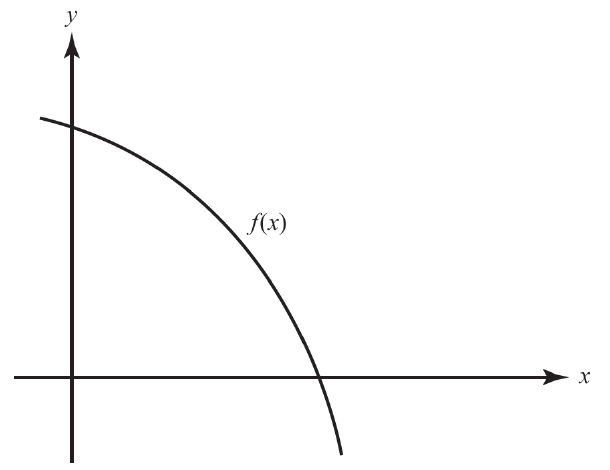
\includegraphics[width=0.6\linewidth]{data/calculus-figures/c4-quadratic.png}\end{center}
\begin{list}{}{\setlength{\leftmargin}{3em}\setlength{\labelwidth}{2.5em}\setlength{\itemsep}{0pt}\setlength{\topsep}{2pt}}
\item[(A)] $c$, $d$, and $e$ are all positive
\item[(B)] $c>0$, $d<0$, $e>0$
\item[(C)] $c<0$, $d>0$, $e>0$
\item[(D)] $c<0$, $d<0$, $e>0$
\end{list}

\bigskip\noindent\textbf{A51.}\ Given $f(x) = \log_{10}x$ and $\log_{10}(102) \approx 2.0086$, which is closest to $f'(100)$?
\begin{list}{}{\setlength{\leftmargin}{3em}\setlength{\labelwidth}{2.5em}\setlength{\itemsep}{0pt}\setlength{\topsep}{2pt}}
\item[(A)] $0.0043$
\item[(B)] $0.0086$
\item[(C)] $0.01$
\item[(D)] $1.0043$
\end{list}

\bigskip\noindent\textbf{B1.}\ The point on $y=\sqrt{2x+1}$ where the tangent is parallel to $x-3y=6$ is
\begin{list}{}{\setlength{\leftmargin}{3em}\setlength{\labelwidth}{2.5em}\setlength{\itemsep}{0pt}\setlength{\topsep}{2pt}}
\item[(A)] $(4,3)$
\item[(B)] $(0,1)$
\item[(C)] $(1,\sqrt3)$
\item[(D)] $(2,\sqrt5)$
\end{list}

\bigskip\noindent\textbf{B2.}\ An equation of the tangent to $x^2=4y$ at the point where $x=-2$ is
\begin{list}{}{\setlength{\leftmargin}{3em}\setlength{\labelwidth}{2.5em}\setlength{\itemsep}{0pt}\setlength{\topsep}{2pt}}
\item[(A)] $x+y-3=0$
\item[(B)] $x-y+3=0$
\item[(C)] $x+y-1=0$
\item[(D)] $x+y+1=0$
\end{list}

\bigskip\noindent\textbf{B3.}\ The table shows velocity at time $t$ for an object moving along a line. Estimate acceleration in ft/sec$^2$ at $t=6$ sec. $\begin{array}{c|rrrr}t\ (\mathrm{sec})&0&4&8&10\\v&18&16&10&0\end{array}$
\begin{list}{}{\setlength{\leftmargin}{3em}\setlength{\labelwidth}{2.5em}\setlength{\itemsep}{0pt}\setlength{\topsep}{2pt}}
\item[(A)] $-6$
\item[(B)] $-1.5$
\item[(C)] $1.5$
\item[(D)] $6$
\end{list}

\bigskip\noindent\textbf{B4.}\ The figure shows $f\prime$ on $[0,7]$. From the graph it follows that
\begin{center}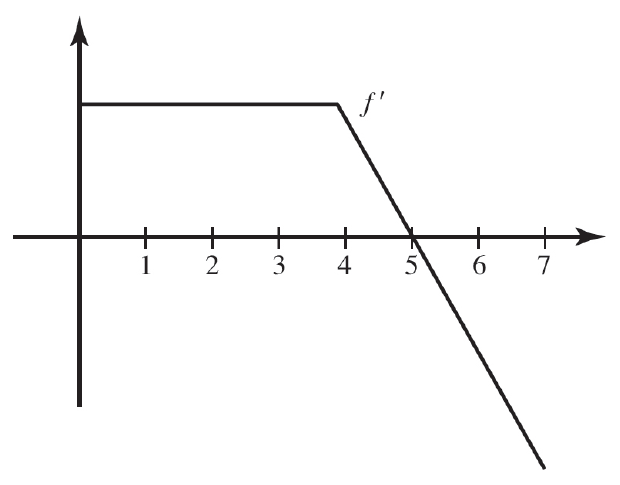
\includegraphics[width=0.6\linewidth]{data/calculus-figures/c4-fprime-linear.png}\end{center}
\begin{list}{}{\setlength{\leftmargin}{3em}\setlength{\labelwidth}{2.5em}\setlength{\itemsep}{0pt}\setlength{\topsep}{2pt}}
\item[(A)] $f$ is discontinuous at $x=4$
\item[(B)] $f$ is decreasing for $4<x<7$
\item[(C)] $f(5) < f(0)$
\item[(D)] $f(2) < f(3)$
\end{list}

\bigskip\noindent\textbf{B5.}\ The figure shows $f\prime$ on $[0,7]$. Which statement best describes $f$ at $x=5$?
\begin{center}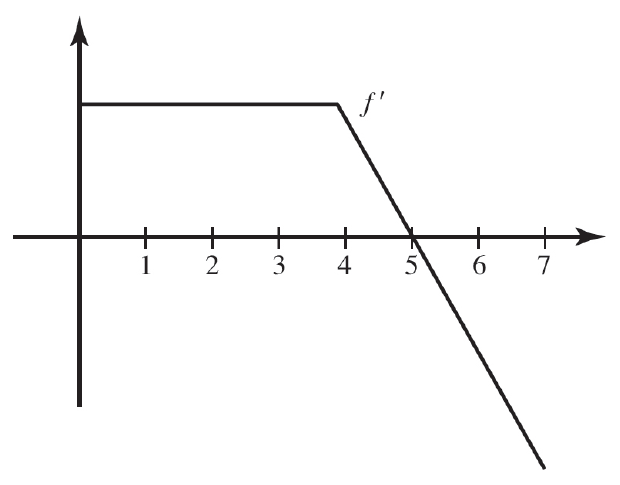
\includegraphics[width=0.6\linewidth]{data/calculus-figures/c4-fprime-linear.png}\end{center}
\begin{list}{}{\setlength{\leftmargin}{3em}\setlength{\labelwidth}{2.5em}\setlength{\itemsep}{0pt}\setlength{\topsep}{2pt}}
\item[(A)] $f$ has a root.
\item[(B)] $f$ has a maximum.
\item[(C)] $f$ has a minimum.
\item[(D)] The graph of $f$ has a point of inflection.
\end{list}

\bigskip\noindent\textbf{B6.}\ The figure shows $f\prime$ on $[0,7]$. For which interval is the graph of $f$ concave downward?
\begin{center}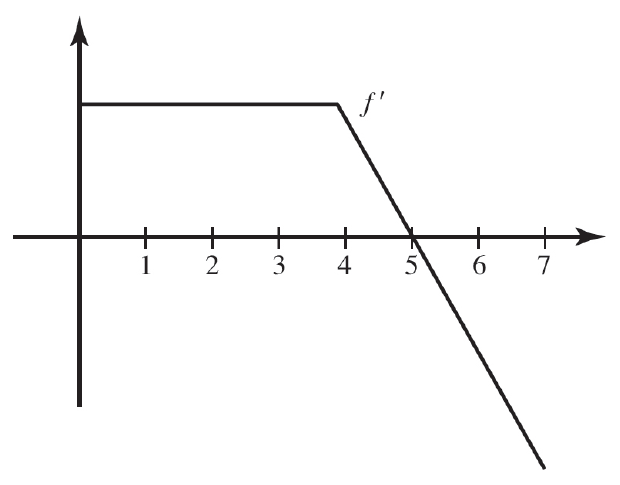
\includegraphics[width=0.6\linewidth]{data/calculus-figures/c4-fprime-linear.png}\end{center}
\begin{list}{}{\setlength{\leftmargin}{3em}\setlength{\labelwidth}{2.5em}\setlength{\itemsep}{0pt}\setlength{\topsep}{2pt}}
\item[(A)] $(0,4)$
\item[(B)] $(4,5)$
\item[(C)] $(5,7)$
\item[(D)] $(4,7)$
\end{list}

\bigskip\noindent\textbf{B7.}\ The figure shows velocity in ft/sec on $0\le t\le5$. The object attains its maximum speed when $t=$
\begin{center}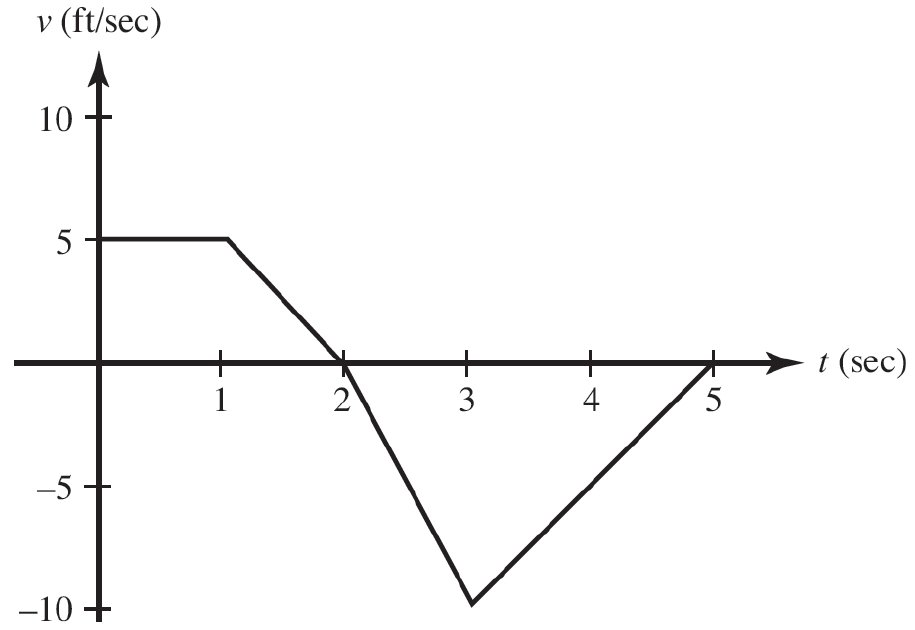
\includegraphics[width=0.6\linewidth]{data/calculus-figures/c4-velocity.png}\end{center}
\begin{list}{}{\setlength{\leftmargin}{3em}\setlength{\labelwidth}{2.5em}\setlength{\itemsep}{0pt}\setlength{\topsep}{2pt}}
\item[(A)] $0$
\item[(B)] $1$
\item[(C)] $2$
\item[(D)] $3$
\end{list}

\bigskip\noindent\textbf{B8.}\ The figure shows velocity in ft/sec on $0\le t\le5$. The speed of the object is increasing during the time interval
\begin{center}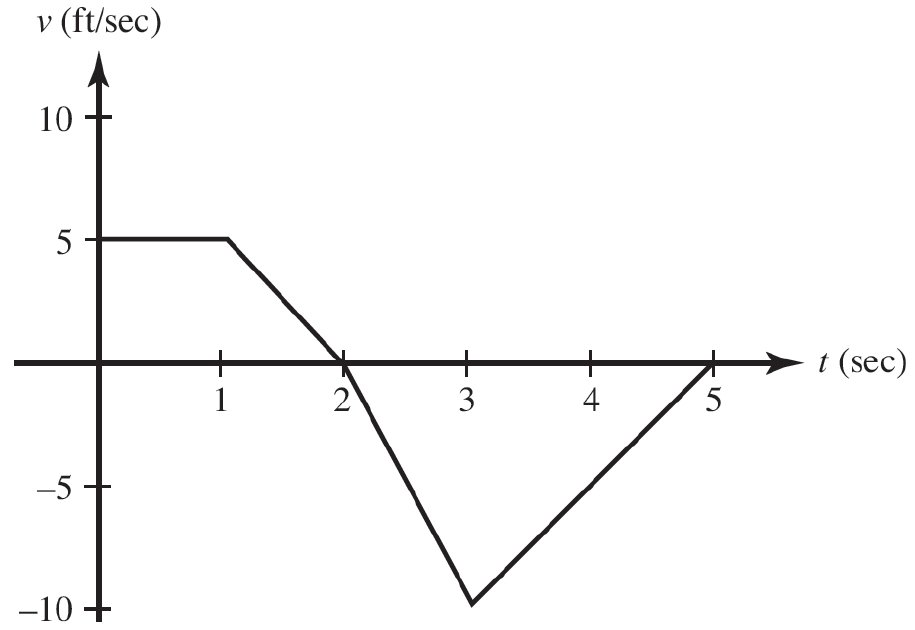
\includegraphics[width=0.6\linewidth]{data/calculus-figures/c4-velocity.png}\end{center}
\begin{list}{}{\setlength{\leftmargin}{3em}\setlength{\labelwidth}{2.5em}\setlength{\itemsep}{0pt}\setlength{\topsep}{2pt}}
\item[(A)] $(1,2)$
\item[(B)] $(0,2)$
\item[(C)] $(2,3)$
\item[(D)] $(3,5)$
\end{list}

\bigskip\noindent\textbf{B9.}\ The figure shows velocity in ft/sec on $0\le t\le5$. The acceleration of the object is positive during the time interval
\begin{center}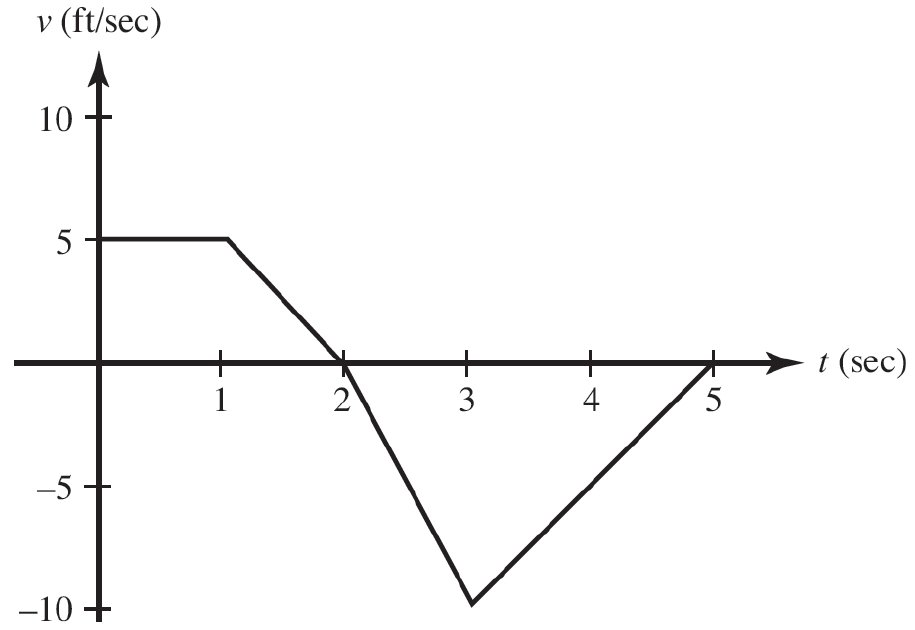
\includegraphics[width=0.6\linewidth]{data/calculus-figures/c4-velocity.png}\end{center}
\begin{list}{}{\setlength{\leftmargin}{3em}\setlength{\labelwidth}{2.5em}\setlength{\itemsep}{0pt}\setlength{\topsep}{2pt}}
\item[(A)] $(1,2)$
\item[(B)] $(0,2)$
\item[(C)] $(2,3)$
\item[(D)] $(3,5)$
\end{list}

\bigskip\noindent\textbf{B10.}\ The figure shows velocity in ft/sec on $0\le t\le5$. How many times on $0<t<5$ is the object's acceleration undefined?
\begin{center}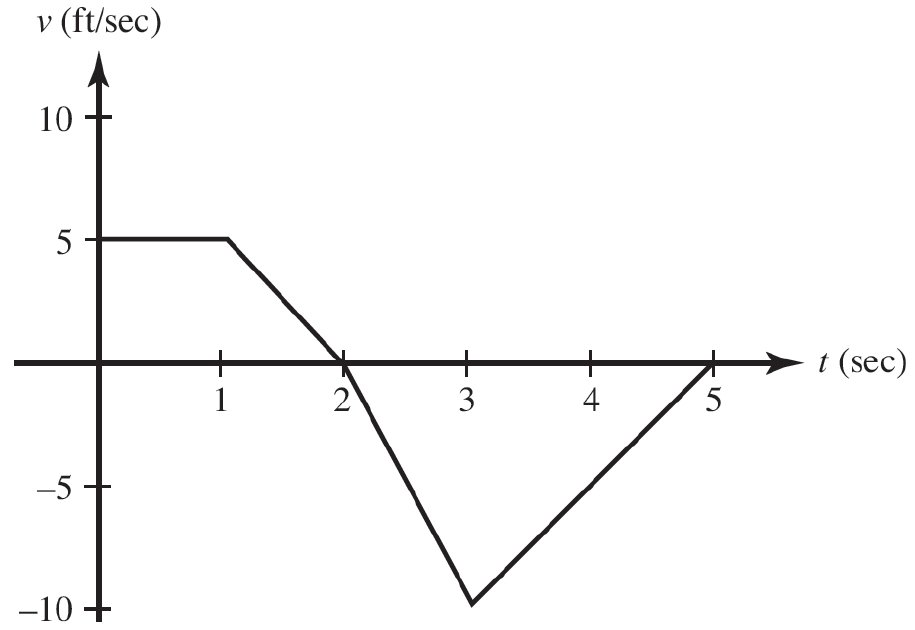
\includegraphics[width=0.6\linewidth]{data/calculus-figures/c4-velocity.png}\end{center}
\begin{list}{}{\setlength{\leftmargin}{3em}\setlength{\labelwidth}{2.5em}\setlength{\itemsep}{0pt}\setlength{\topsep}{2pt}}
\item[(A)] none
\item[(B)] $1$
\item[(C)] $2$
\item[(D)] $3$
\end{list}

\bigskip\noindent\textbf{B11.}\ The figure shows velocity in ft/sec on $0\le t\le5$. During $2<t<3$, the object's acceleration (in ft/sec$^2$) is
\begin{center}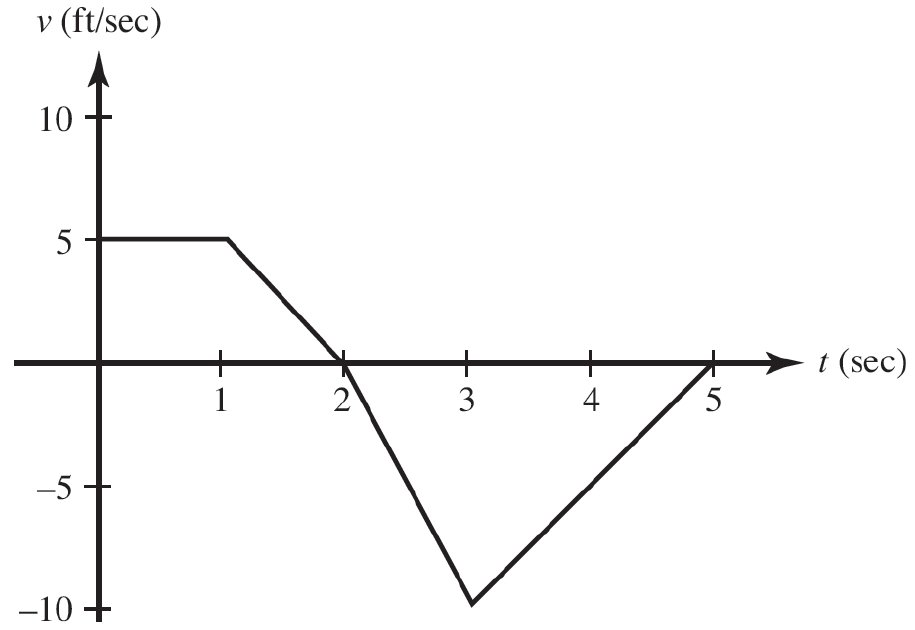
\includegraphics[width=0.6\linewidth]{data/calculus-figures/c4-velocity.png}\end{center}
\begin{list}{}{\setlength{\leftmargin}{3em}\setlength{\labelwidth}{2.5em}\setlength{\itemsep}{0pt}\setlength{\topsep}{2pt}}
\item[(A)] $-10$
\item[(B)] $-5$
\item[(C)] $5$
\item[(D)] $10$
\end{list}

\bigskip\noindent\textbf{B12.}\ The figure shows velocity in ft/sec on $0\le t\le5$. The object is farthest to the right when $t=$
\begin{center}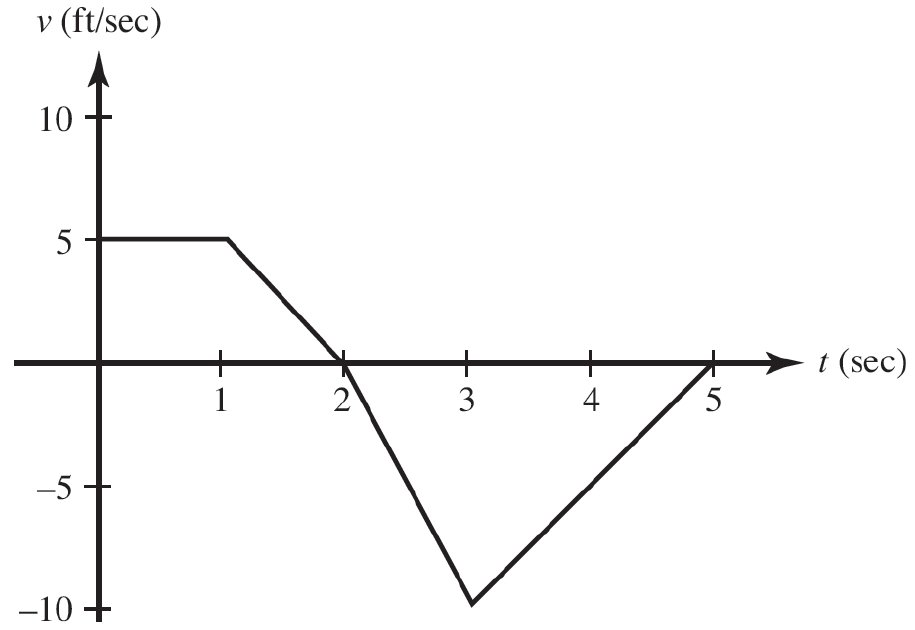
\includegraphics[width=0.6\linewidth]{data/calculus-figures/c4-velocity.png}\end{center}
\begin{list}{}{\setlength{\leftmargin}{3em}\setlength{\labelwidth}{2.5em}\setlength{\itemsep}{0pt}\setlength{\topsep}{2pt}}
\item[(A)] $0$
\item[(B)] $1$
\item[(C)] $2$
\item[(D)] $5$
\end{list}

\bigskip\noindent\textbf{B13.}\ The figure shows velocity in ft/sec on $0\le t\le5$. The object's average acceleration (in ft/sec$^2$) for the interval $0 \leq t \leq 3$ is
\begin{center}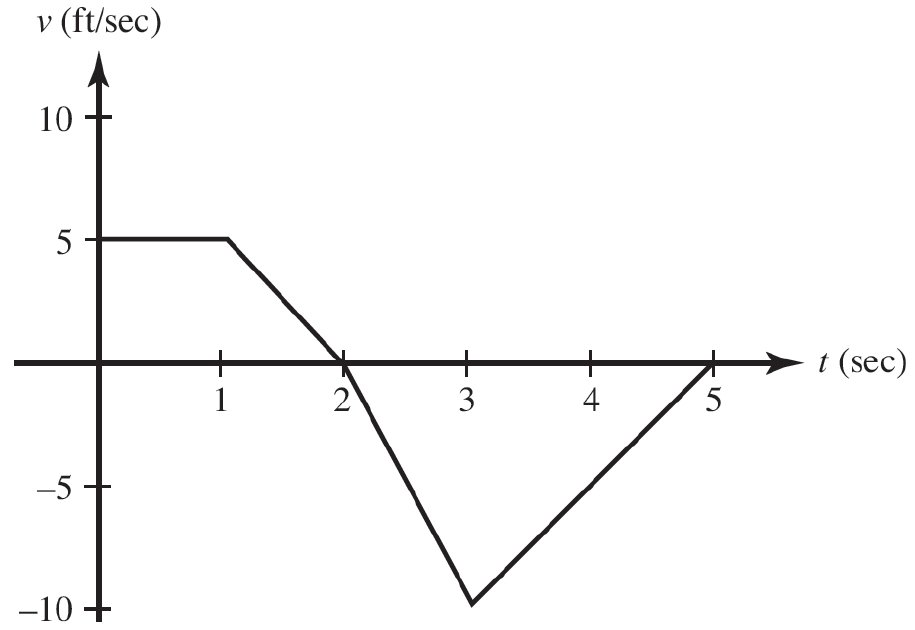
\includegraphics[width=0.6\linewidth]{data/calculus-figures/c4-velocity.png}\end{center}
\begin{list}{}{\setlength{\leftmargin}{3em}\setlength{\labelwidth}{2.5em}\setlength{\itemsep}{0pt}\setlength{\topsep}{2pt}}
\item[(A)] $-15$
\item[(B)] $-5$
\item[(C)] $-3$
\item[(D)] $-1$
\end{list}

\bigskip\noindent\textbf{B14.}\ The line $y=3x+k$ is tangent to the curve $y=x^3$ when $k$ is equal to
\begin{list}{}{\setlength{\leftmargin}{3em}\setlength{\labelwidth}{2.5em}\setlength{\itemsep}{0pt}\setlength{\topsep}{2pt}}
\item[(A)] $1$ or $-1$
\item[(B)] $2$ or $-2$
\item[(C)] $3$ or $-3$
\item[(D)] $4$ or $-4$
\end{list}

\bigskip\noindent\textbf{B15.}\ The two tangents that can be drawn from the point $(3,5)$ to the parabola $y=x^2$ have slopes
\begin{list}{}{\setlength{\leftmargin}{3em}\setlength{\labelwidth}{2.5em}\setlength{\itemsep}{0pt}\setlength{\topsep}{2pt}}
\item[(A)] $1$ and $5$
\item[(B)] $0$ and $4$
\item[(C)] $2$ and $10$
\item[(D)] $2$ and $4$
\end{list}

\bigskip\noindent\textbf{B16.}\ The table shows velocity for an object moving along a line. Estimate acceleration in ft/sec$^2$ at $t=1$. $\begin{array}{c|rrrr}t\ (\mathrm{sec})&1.0&1.5&2.2&2.5\\v\ (\mathrm{ft/sec})&12.2&13.0&13.4&13.7\end{array}$
\begin{list}{}{\setlength{\leftmargin}{3em}\setlength{\labelwidth}{2.5em}\setlength{\itemsep}{0pt}\setlength{\topsep}{2pt}}
\item[(A)] $0.8$
\item[(B)] $1.0$
\item[(C)] $1.2$
\item[(D)] $1.6$
\end{list}

\bigskip\noindent\textbf{B17.}\ For $0<x<4$, $f\prime(x)=x\sin x-\cos x$. $f$ has a local maximum when $x$ is approximately
\begin{list}{}{\setlength{\leftmargin}{3em}\setlength{\labelwidth}{2.5em}\setlength{\itemsep}{0pt}\setlength{\topsep}{2pt}}
\item[(A)] $1.192$
\item[(B)] $2.289$
\item[(C)] $3.426$
\item[(D)] $3.809$
\end{list}

\bigskip\noindent\textbf{B18.}\ For $0<x<4$, $f\prime(x)=x\sin x-\cos x$. The graph of $f$ has a point of inflection when $x$ is approximately
\begin{list}{}{\setlength{\leftmargin}{3em}\setlength{\labelwidth}{2.5em}\setlength{\itemsep}{0pt}\setlength{\topsep}{2pt}}
\item[(A)] $1.192$
\item[(B)] $2.289$
\item[(C)] $3.426$
\item[(D)] $3.809$
\end{list}

\bigskip\noindent\textbf{B19.}\ A particle has position $x=2t$, $y=4t-t^2$. The particle moves along
\begin{list}{}{\setlength{\leftmargin}{3em}\setlength{\labelwidth}{2.5em}\setlength{\itemsep}{0pt}\setlength{\topsep}{2pt}}
\item[(A)] an ellipse
\item[(B)] a hyperbola
\item[(C)] a line
\item[(D)] a parabola
\end{list}

\bigskip\noindent\textbf{B20.}\ A particle has position $x=2t$, $y=4t-t^2$. The speed of the particle at any time $t$ is
\begin{list}{}{\setlength{\leftmargin}{3em}\setlength{\labelwidth}{2.5em}\setlength{\itemsep}{0pt}\setlength{\topsep}{2pt}}
\item[(A)] $\sqrt{6-2t}$
\item[(B)] $2\sqrt{t^2-4t+5}$
\item[(C)] $2\sqrt{t^2-2t+5}$
\item[(D)] $2|3-t|$
\end{list}

\bigskip\noindent\textbf{B21.}\ A particle has position $x=2t$, $y=4t-t^2$. The minimum speed of the particle is
\begin{list}{}{\setlength{\leftmargin}{3em}\setlength{\labelwidth}{2.5em}\setlength{\itemsep}{0pt}\setlength{\topsep}{2pt}}
\item[(A)] $0$
\item[(B)] $1$
\item[(C)] $2$
\item[(D)] $4$
\end{list}

\bigskip\noindent\textbf{B22.}\ A particle has position $x=2t$, $y=4t-t^2$. The acceleration of the particle
\begin{list}{}{\setlength{\leftmargin}{3em}\setlength{\labelwidth}{2.5em}\setlength{\itemsep}{0pt}\setlength{\topsep}{2pt}}
\item[(A)] depends on $t$
\item[(B)] is always directed upward
\item[(C)] is constant both in magnitude and in direction
\item[(D)] never exceeds 1 in magnitude
\end{list}

\bigskip\noindent\textbf{B23.}\ If a particle moves along a curve with constant speed, then
\begin{list}{}{\setlength{\leftmargin}{3em}\setlength{\labelwidth}{2.5em}\setlength{\itemsep}{0pt}\setlength{\topsep}{2pt}}
\item[(A)] the magnitude of its acceleration must equal zero
\item[(B)] the direction of acceleration must be constant
\item[(C)] the curve along which the particle moves must be a straight line
\item[(D)] its velocity and acceleration vectors must be perpendicular
\end{list}

\bigskip\noindent\textbf{B24.}\ A particle moves on $y=2x-\ln x$ with $dx/dt=-2$ at all times. At $(1,2)$, $dy/dt$ is
\begin{list}{}{\setlength{\leftmargin}{3em}\setlength{\labelwidth}{2.5em}\setlength{\itemsep}{0pt}\setlength{\topsep}{2pt}}
\item[(A)] $-4$
\item[(B)] $-2$
\item[(C)] $2$
\item[(D)] $4$
\end{list}

\bigskip\noindent\textbf{B25.}\ A particle moves on $r=6\cos2\theta$, with $d\theta/dt=1/3$ radian/sec when $\theta=\pi/6$. At $\theta = \dfrac{\pi}{6}$, find the rate of change (in units per second) of the particle's distance from the origin.
\begin{list}{}{\setlength{\leftmargin}{3em}\setlength{\labelwidth}{2.5em}\setlength{\itemsep}{0pt}\setlength{\topsep}{2pt}}
\item[(A)] $-6\sqrt3$
\item[(B)] $-2\sqrt3$
\item[(C)] $2\sqrt3$
\item[(D)] $6\sqrt3$
\end{list}

\bigskip\noindent\textbf{B26.}\ A particle moves on $r=6\cos2\theta$, with $d\theta/dt=1/3$ radian/sec when $\theta=\pi/6$. At $\theta = \dfrac{\pi}{6}$, what is the horizontal component of the particle's velocity?
\begin{list}{}{\setlength{\leftmargin}{3em}\setlength{\labelwidth}{2.5em}\setlength{\itemsep}{0pt}\setlength{\topsep}{2pt}}
\item[(A)] $-\dfrac{21}{2}$
\item[(B)] $-\dfrac{7}{2}$
\item[(C)] $-2$
\item[(D)] $\dfrac{1}{2}$
\end{list}

\bigskip\noindent\textbf{B27.}\ The figure shows $f\prime$ on $[0,5]$. $f$ has a local minimum at $x=$
\begin{center}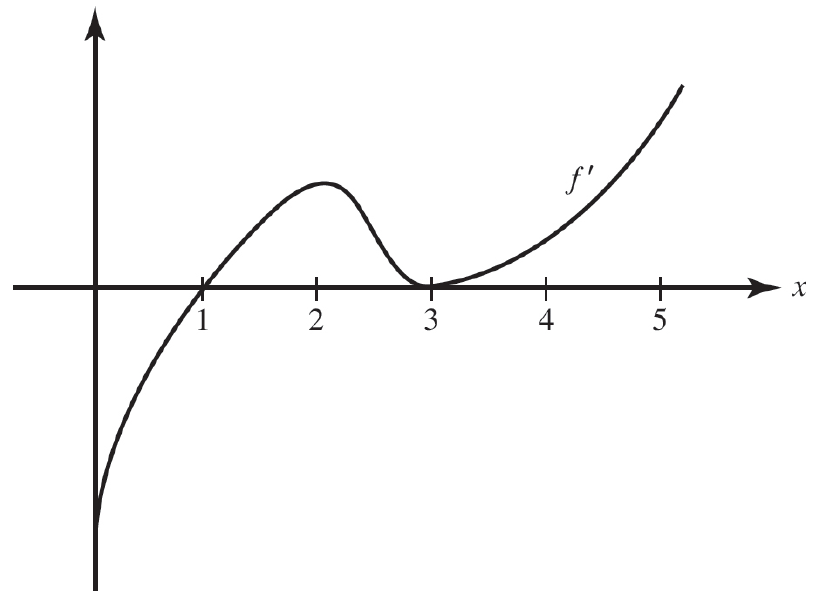
\includegraphics[width=0.6\linewidth]{data/calculus-figures/c4-fprime-turns.png}\end{center}
\begin{list}{}{\setlength{\leftmargin}{3em}\setlength{\labelwidth}{2.5em}\setlength{\itemsep}{0pt}\setlength{\topsep}{2pt}}
\item[(A)] $0$
\item[(B)] $1$
\item[(C)] $2$
\item[(D)] $3$
\end{list}

\bigskip\noindent\textbf{B28.}\ The figure shows $f\prime$ on $[0,5]$. The graph of $f$ has a point of inflection at $x=$
\begin{center}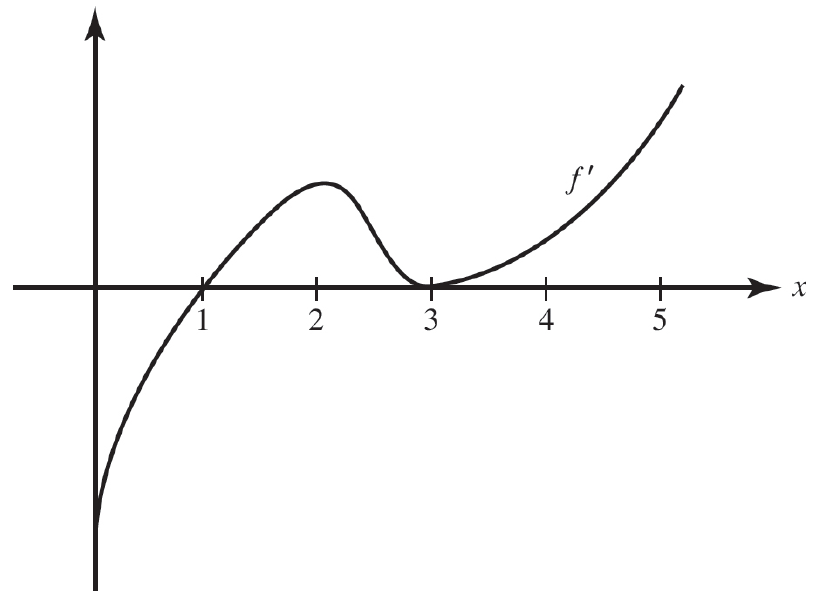
\includegraphics[width=0.6\linewidth]{data/calculus-figures/c4-fprime-turns.png}\end{center}
\begin{list}{}{\setlength{\leftmargin}{3em}\setlength{\labelwidth}{2.5em}\setlength{\itemsep}{0pt}\setlength{\topsep}{2pt}}
\item[(A)] $1$ only
\item[(B)] $2$ only
\item[(C)] $3$ only
\item[(D)] $2$ and $3$ only
\end{list}

\bigskip\noindent\textbf{B29.}\ It follows from the graph of $f\prime$, shown below, that
\begin{center}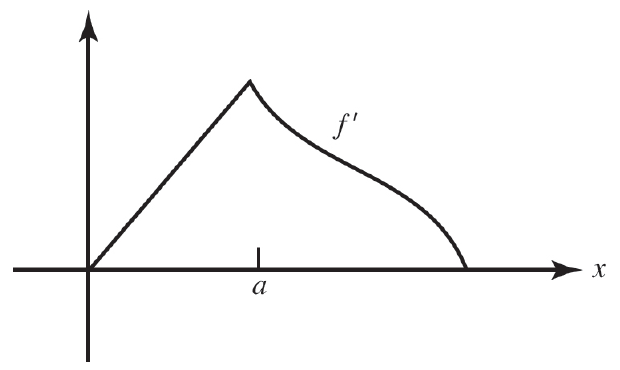
\includegraphics[width=0.6\linewidth]{data/calculus-figures/c4-fprime-corner.png}\end{center}
\begin{list}{}{\setlength{\leftmargin}{3em}\setlength{\labelwidth}{2.5em}\setlength{\itemsep}{0pt}\setlength{\topsep}{2pt}}
\item[(A)] $f$ is not continuous at $x=a$
\item[(B)] $f$ is continuous but not differentiable at $x=a$
\item[(C)] $f$ has a relative maximum at $x=a$
\item[(D)] The graph of $f$ has a point of inflection at $x=a$
\end{list}

\bigskip\noindent\textbf{B30.}\ A vertical circular cylinder has radius $r$ ft and height $h$ ft. If the height and radius both increase at the constant rate of 2 ft/sec, then the rate, in square feet per second, at which the lateral surface area increases is
\begin{list}{}{\setlength{\leftmargin}{3em}\setlength{\labelwidth}{2.5em}\setlength{\itemsep}{0pt}\setlength{\topsep}{2pt}}
\item[(A)] $4\pi r$
\item[(B)] $2\pi(r+h)$
\item[(C)] $4\pi(r+h)$
\item[(D)] $4\pi h$
\end{list}

\bigskip\noindent\textbf{B31.}\ A tangent drawn to the parabola $y=4-x^2$ at the point $(1,3)$ forms a right triangle with the coordinate axes. The area of the triangle is
\begin{list}{}{\setlength{\leftmargin}{3em}\setlength{\labelwidth}{2.5em}\setlength{\itemsep}{0pt}\setlength{\topsep}{2pt}}
\item[(A)] $\frac54$
\item[(B)] $\frac52$
\item[(C)] $\frac{25}2$
\item[(D)] $\frac{25}4$
\end{list}

\bigskip\noindent\textbf{B32.}\ Two cars are traveling along perpendicular roads, car $A$ at 40 mph and car $B$ at 60 mph. At noon, when car $A$ reaches the intersection, car $B$ is 90 miles away, and moving toward the intersection. At 1 P.M. the rate, in miles per hour, at which the distance between the cars is changing is
\begin{list}{}{\setlength{\leftmargin}{3em}\setlength{\labelwidth}{2.5em}\setlength{\itemsep}{0pt}\setlength{\topsep}{2pt}}
\item[(A)] $-68$
\item[(B)] $-4$
\item[(C)] $4$
\item[(D)] $68$
\end{list}

\bigskip\noindent\textbf{B33.}\ Two cars are traveling along perpendicular roads, car $A$ at 40 mph and car $B$ at 60 mph. At noon, when car $A$ reaches the intersection, car $B$ is 90 miles away and moving toward the intersection. If $t$ represents the time, in hours, traveled after noon, then the cars are closest together when $t$ is
\begin{list}{}{\setlength{\leftmargin}{3em}\setlength{\labelwidth}{2.5em}\setlength{\itemsep}{0pt}\setlength{\topsep}{2pt}}
\item[(A)] $1.038$
\item[(B)] $1.077$
\item[(C)] $1.5$
\item[(D)] $1.8$
\end{list}

\bigskip\noindent\textbf{B34.}\ The figure shows velocity in ft/sec on $0\le t\le12$. For what $t$ does this object attain its maximum acceleration?
\begin{center}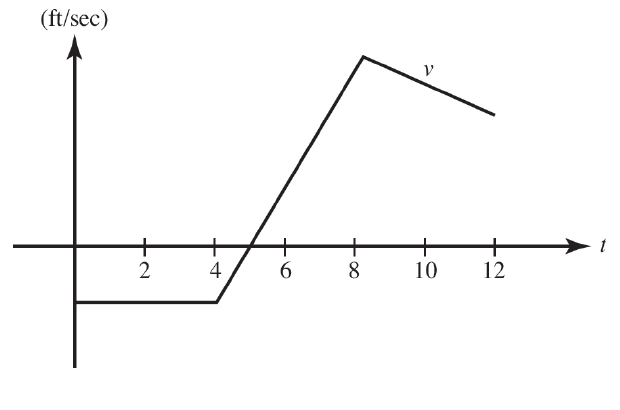
\includegraphics[width=0.6\linewidth]{data/calculus-figures/c4-velocity-long.png}\end{center}
\begin{list}{}{\setlength{\leftmargin}{3em}\setlength{\labelwidth}{2.5em}\setlength{\itemsep}{0pt}\setlength{\topsep}{2pt}}
\item[(A)] $0<t<4$
\item[(B)] $4<t<8$
\item[(C)] $t=5$
\item[(D)] $t=8$
\end{list}

\bigskip\noindent\textbf{B35.}\ The figure shows velocity in ft/sec on $0\le t\le12$. The object reverses direction at $t=$
\begin{center}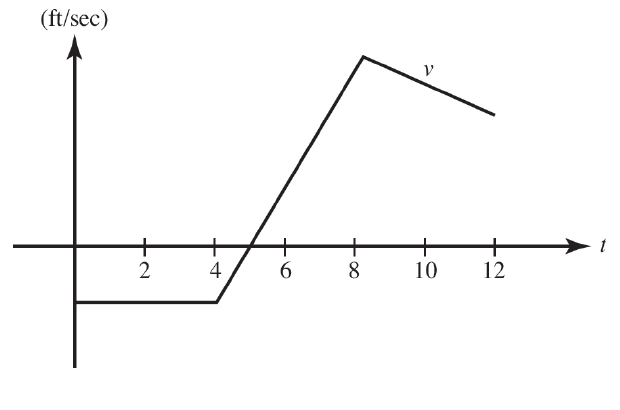
\includegraphics[width=0.6\linewidth]{data/calculus-figures/c4-velocity-long.png}\end{center}
\begin{list}{}{\setlength{\leftmargin}{3em}\setlength{\labelwidth}{2.5em}\setlength{\itemsep}{0pt}\setlength{\topsep}{2pt}}
\item[(A)] $4$ only
\item[(B)] $5$ only
\item[(C)] $8$ only
\item[(D)] $5$ and $8$
\end{list}

\bigskip\noindent\textbf{B36.}\ Given $f\prime$ as graphed, which could be the graph of $f$?
\begin{center}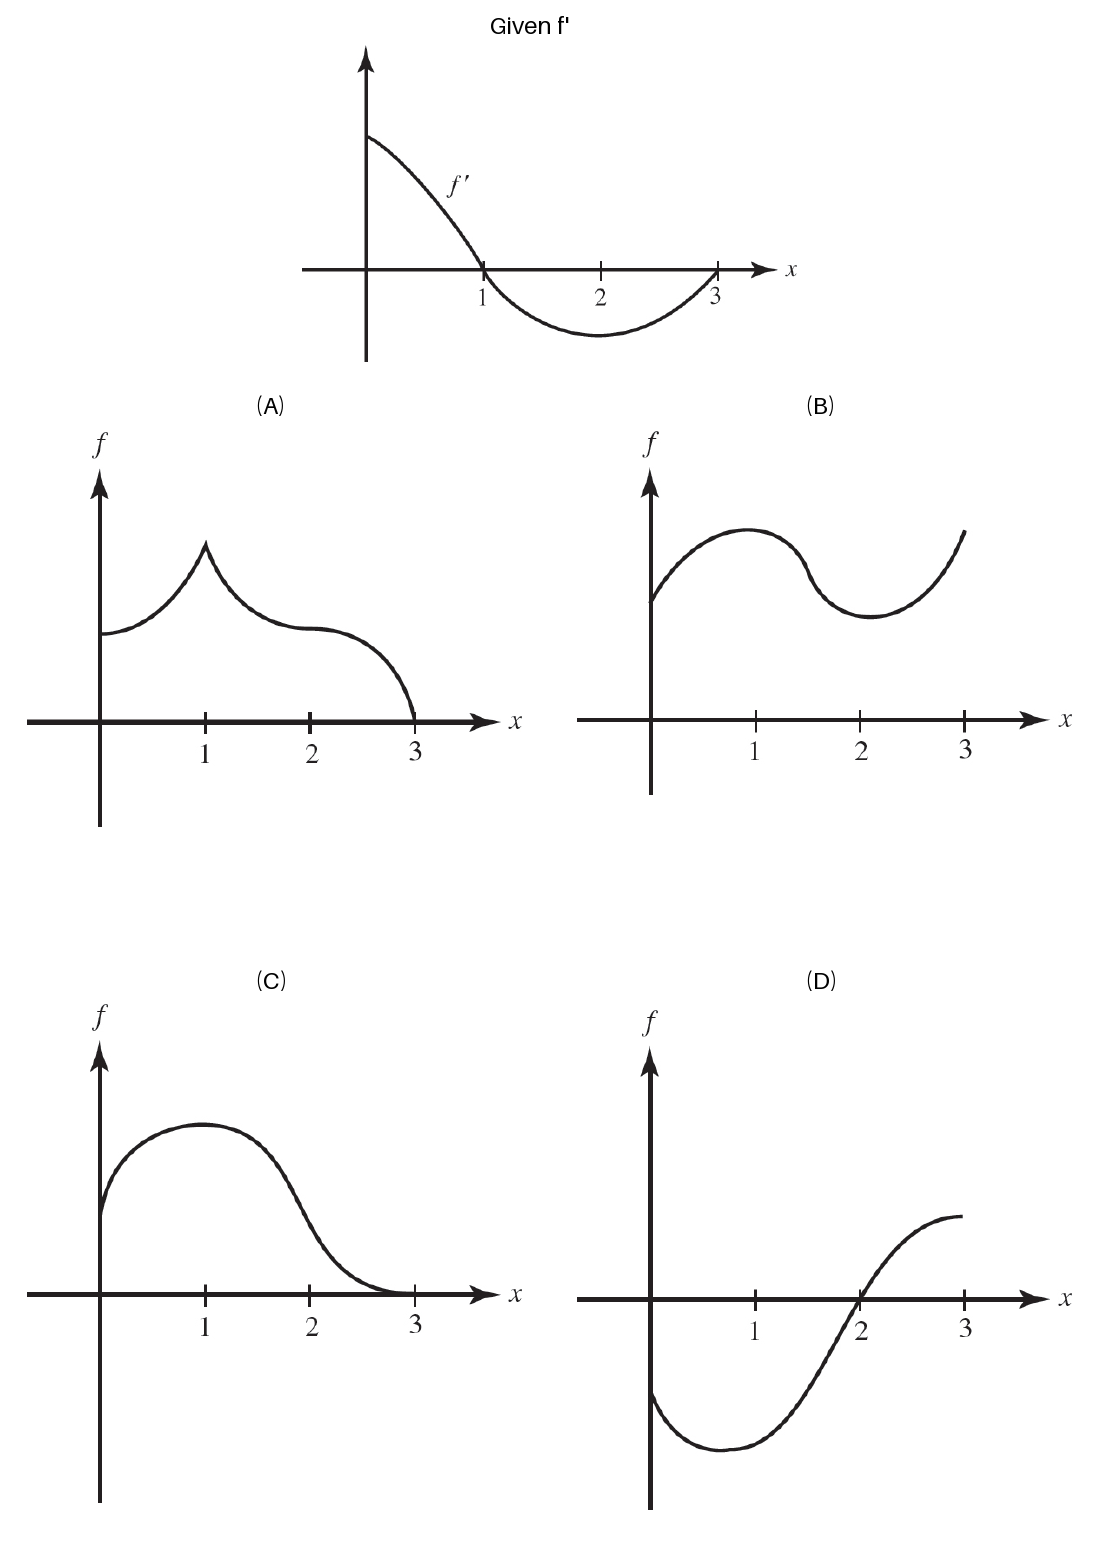
\includegraphics[width=0.6\linewidth]{data/calculus-figures/c4-function-choices.png}\end{center}
\begin{list}{}{\setlength{\leftmargin}{3em}\setlength{\labelwidth}{2.5em}\setlength{\itemsep}{0pt}\setlength{\topsep}{2pt}}
\item[(A)] Graph (A)
\item[(B)] Graph (B)
\item[(C)] Graph (C)
\item[(D)] Graph (D)
\end{list}

\bigskip\noindent\textbf{B37.}\ The graph of $f\prime$ is shown. If $f(2)=10$, the local linearization of $f$ at $x=2$ is $f(x)\approx$
\begin{center}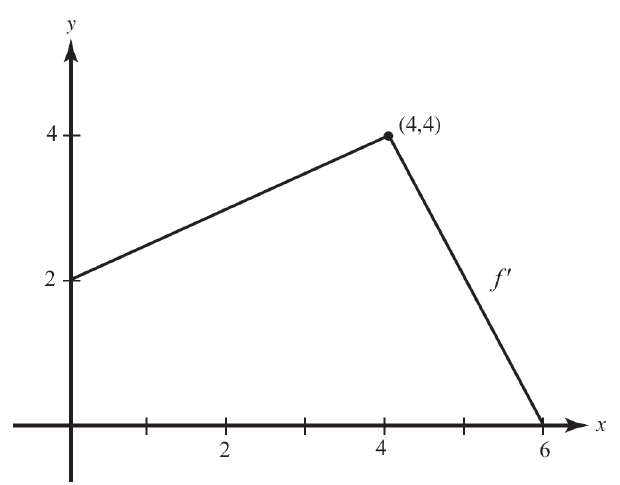
\includegraphics[width=0.6\linewidth]{data/calculus-figures/c4-linearization.png}\end{center}
\begin{list}{}{\setlength{\leftmargin}{3em}\setlength{\labelwidth}{2.5em}\setlength{\itemsep}{0pt}\setlength{\topsep}{2pt}}
\item[(A)] $\frac x2+2$
\item[(B)] $\frac x2+9$
\item[(C)] $3x-3$
\item[(D)] $3x+4$
\end{list}

\bigskip\noindent\textbf{B38.}\ Use the labeled curve in the figure. At which labeled point do both $\dfrac{dy}{dx}$ and $\dfrac{d^2y}{dx^2}$ equal zero?
\begin{center}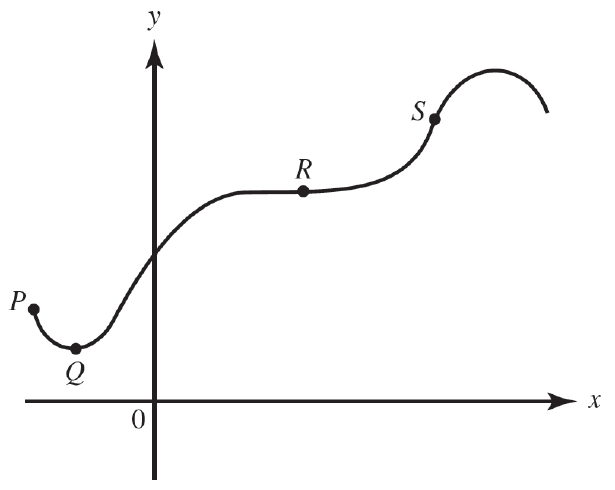
\includegraphics[width=0.6\linewidth]{data/calculus-figures/c4-labeled-curve.png}\end{center}
\begin{list}{}{\setlength{\leftmargin}{3em}\setlength{\labelwidth}{2.5em}\setlength{\itemsep}{0pt}\setlength{\topsep}{2pt}}
\item[(A)] $P$
\item[(B)] $Q$
\item[(C)] $R$
\item[(D)] $S$
\end{list}

\bigskip\noindent\textbf{B39.}\ Use the labeled curve in the figure. At which labeled point is $\dfrac{dy}{dx}$ positive and $\dfrac{d^2y}{dx^2}$ equal to zero?
\begin{center}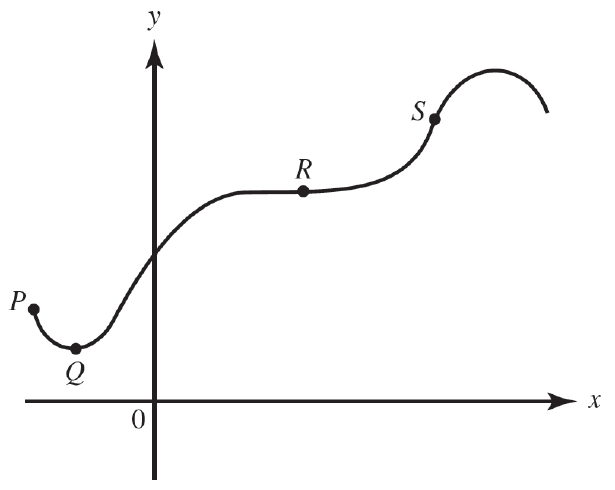
\includegraphics[width=0.6\linewidth]{data/calculus-figures/c4-labeled-curve.png}\end{center}
\begin{list}{}{\setlength{\leftmargin}{3em}\setlength{\labelwidth}{2.5em}\setlength{\itemsep}{0pt}\setlength{\topsep}{2pt}}
\item[(A)] $P$
\item[(B)] $Q$
\item[(C)] $R$
\item[(D)] $S$
\end{list}

\bigskip\noindent\textbf{B40.}\ Use the labeled curve in the figure. At which labeled point is $\dfrac{dy}{dx}$ equal to zero and $\dfrac{d^2y}{dx^2}$ positive?
\begin{center}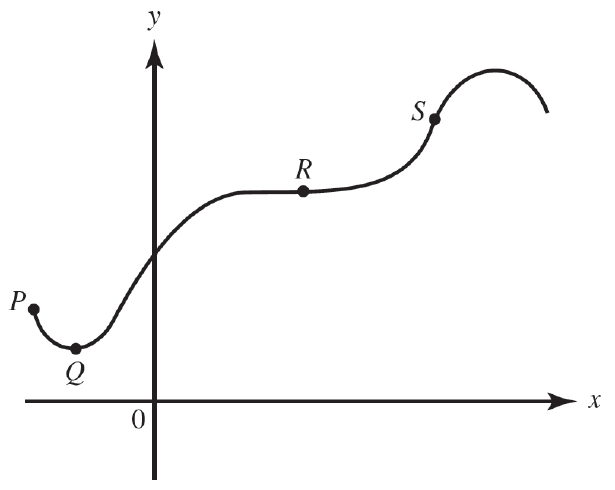
\includegraphics[width=0.6\linewidth]{data/calculus-figures/c4-labeled-curve.png}\end{center}
\begin{list}{}{\setlength{\leftmargin}{3em}\setlength{\labelwidth}{2.5em}\setlength{\itemsep}{0pt}\setlength{\topsep}{2pt}}
\item[(A)] $P$
\item[(B)] $Q$
\item[(C)] $R$
\item[(D)] $S$
\end{list}

\bigskip\noindent\textbf{B41.}\ If $f(6)=30$ and $f\prime(x)=x^2/(x+3)$, estimate $f(6.02)$ using the tangent line at $x=6$.
\begin{list}{}{\setlength{\leftmargin}{3em}\setlength{\labelwidth}{2.5em}\setlength{\itemsep}{0pt}\setlength{\topsep}{2pt}}
\item[(A)] $29.92$
\item[(B)] $30.02$
\item[(C)] $30.08$
\item[(D)] $30.16$
\end{list}

\bigskip\noindent\textbf{B42.}\ A local linear approximation for $f(x)=\sqrt{x^2+16}$ near $x=-3$ is
\begin{list}{}{\setlength{\leftmargin}{3em}\setlength{\labelwidth}{2.5em}\setlength{\itemsep}{0pt}\setlength{\topsep}{2pt}}
\item[(A)] $y=5-\frac35(x-3)$
\item[(B)] $y=5+\frac35(x-3)$
\item[(C)] $y=5-\frac35(x+3)$
\item[(D)] $y=3-\frac53(x-3)$
\end{list}

\end{document}
